\documentclass{article}

\usepackage{geometry}
 \geometry{
 a4paper,
 total={170mm,257mm},
 left=20mm,
 top=20mm
 }
\usepackage{float}
\usepackage{graphicx}
\usepackage{indentfirst}
\usepackage{hyperref}

\usepackage{tikz}
\usetikzlibrary{shapes.geometric, arrows}

\tikzstyle{startstop} = [rectangle, rounded corners, minimum width=3cm, minimum height=1cm,text centered, draw=black, fill=red!30]
\tikzstyle{io} = [trapezium, trapezium left angle=70, trapezium right angle=110, minimum width=2.5cm, minimum height=1cm, text centered, draw=black, fill=blue!30, text width=2cm]
\tikzstyle{process} = [rectangle, minimum width=3cm, minimum height=1cm, text centered, draw=black, fill=orange!30]
\tikzstyle{decision} = [diamond, minimum width=3cm, minimum height=1cm, text centered, draw=black, fill=green!30]
\tikzstyle{arrow} = [thick,->,>=stealth]
\tikzstyle{double-arrow} = [thick,<->,>=stealth]

\usepackage[backend=biber]{biblatex}
\addbibresource{daftar_pustaka.bib}
\graphicspath{ {./images/} }
\renewcommand*\contentsname{Daftar Isi}
\renewcommand{\figurename}{Figur}
\renewcommand{\tablename}{Tabel}

\begin{document}
  \begin{titlepage}
    \begin{center}
      
      \null
      {
      \huge \bfseries MAKALAH}\\
      [1cm]
      {\LARGE Deteksi COVID-19 pada Dataset X-Ray Dada dengan Metode Capsule Neural Network (CapsNet)}\\
          
      \vspace{2cm}

      \begin{figure}[H]
        \centering
        \includegraphics[width=200px]{/logo/Lambang UGM.jpg}
      \end{figure}
          
      \vspace{3cm}
    
      {\Large 
      Disusun oleh Tim \bfseries Yakuy 2} {\Large :\\
      \vspace{0.5cm}
      Ardacandra Subiantoro (18/427572/PA/18532)\\
      Arief Pujo Arianto (18/430253/PA/18766)\\
      Chrystian (18/430257/PA/18770)\\
      }


      \vspace{2cm}

      {\normalsize \bfseries
      PROGRAM STUDI S1 ILMU KOMPUTER\\
      DEPARTEMEN ILMU KOMPUTER DAN ELEKTRONIKA\\
      FAKULTAS MATEMATIKA DAN ILMU PENGETAHUAN ALAM\\
      UNIVERSITAS GADJAH MADA\\
      YOGYAKARTA\\
      \vspace{0.2cm}
      2020
      }
            
    \end{center}
  \end{titlepage}

  \pagenumbering{gobble}

  \newpage
  \pagenumbering{arabic}
  \tableofcontents
  \newpage
  \section{Pendahuluan}
	  \subsection{Latar Belakang}
	   Jumlah kasus COVID-19 terus meningkat secara eksponensial. Jumlah kasus total COVID-19 di seluruh dunia sudah mencapai lebih dari 19 juta kasus, dengan lebih dari 700 ribu kematian akibat COVID-19. Kasus COVID-19 di Indonesia sudah mencapai lebih dari 120 ribu dengan lebih dari 5 ribu kematian. Dampak negatif dari pandemi COVID-19 ini sangat terasa di Indonesia. Direktur Jenderal Pajak Kementerian Keuangan (Kemenkeu) Suryo Utomo membagi dampak pandemi COVID-19 menjadi tiga garis besar \cite{zuraya}. Dampak pertama adalah membuat konsumsi rumah tangga atau daya beli yang merupakan penopang 60 \% terhadap ekonomi jatuh cukup dalam. Hal ini dibuktikan dengan data dari BPS yang mencatatkan bahwa konsumsi rumah tangga turun dari 5,02 \% pada kuartal I 2019 ke 2,84 \% pada kuartal I tahun ini. Dampak kedua yaitu pandemi menimbulkan adanya ketidakpastian yang berkepanjangan sehingga investasi ikut melemah dan berimplikasi pada terhentinya usaha. Dampak ketiga adalah seluruh dunia mengalami pelemahan ekonomi sehingga menyebabkan harga komoditas turun dan ekspor Indonesia ke beberapa negara juga terhenti. 
	   \par
	   Jumlah alat testing yang terbatas membuat tidak mungkin setiap pasien dengan penyakit pernafasan untuk dites dengan teknik konvensional (RT-PCR) untuk mendeteksi COVID-19. Jumlah ruang di rumah sakit, jumlah ventilator, dan jumlah alat protektif (PPE) bagi tenaga medis sangat terbatas, sehingga perlu digunakan dengan seefisien mungkin. Untuk meningkatkan efisiensi penggunaan alat medis, sangat penting untuk dapat membedakan pasien dengan \textit{severe acute respiratory illness} (SARI) yang mungkin terinfeksi COVID-19. Oleh karena itu, kami mencoba menggunakan gambar X-Ray dada untuk mendeteksi infeksi COVID-19 dengan metode CapsNet.
	   Penggunaan gambar X-Ray memiliki beberapa keuntungan dibandingkan tes konvensional \cite{mangal} :
	   
	   \begin{enumerate}
	   	\item Pengambilan gambar X-Ray lebih banyak digunakan dan lebih murah dibandingkan tes konvensional.
	   	\item Gambar X-Ray dapat dengan mudah ditransfer tanpa perlu ada alat transportasi dari tempat pengambilan gambar ke tempat analisis gambar, sehingga proses diagnostik dapat dilaksanakan dengan cepat.
	   	\item Berbeda dengan CT Scan, terdapat alat-alat pengambil gambar X-Ray portable sehingga tes dapat dilakukan di ruangan-ruangan isolasi. Hal ini menyebabkan kurangnya penggunaan alat-alat protektif dan mengurangi risiko infeksi tersebar ke pasien-pasien lain di rumah sakit.
	   \end{enumerate}
	 
	   Dataset yang akan kami gunakan berasal dari dua sumber. Sumber pertama adalah  Kaggle Chest X-Ray Images (Pneumonia) dataset (2018) milik Paul Mooney \cite{mooney} yang berisi 5,863 gambar X-Ray dada yang dipilih dari pasien-pasien anak berumur satu sampai lima tahun dari Guangzhou Women and Children’s Medical Center, Guangzhou. Paul Mooney mendapatkan data tersebut dari \textit{paper} "Labeled Optical Coherence Tomography (OCT) and Chest X-Ray Images for Classification" karya Kermany, D., Zhang, K., dan Goldbaum, M. \cite{kermany}.Sumber kedua adalah dari \textit{repository} Covid-19 Image Data Collection milik Cohen, J.P., Morrison, P., dan Dao, L. \cite{cohen} yang berisi 454 gambar X-Ray dada pasien dengan penyakit paru-paru termasuk COVID-19 dan juga metadata yang mendeskripsikan informasi-informasi seperti jenis kelamin, umur, lokasi, dll dari pasien. 
	   
	   \subsection{Tujuan dan Manfaat}
	   Tujuan utama kami adalah untuk mengusulkan model berbasis \textit{neural network} yang dapat secara akurat mendeteksi infeksi COVID-19 dari gambar X-Ray dada pasien. Model ini diharapkan dapat bertindak sebagai alat otomatis yang dapat memandu petugas kesehatan dalam mendiagnosis gambar X-Ray agar mengambil kesimpulan yang akurat. Manfaat yang diharapkan adalah peningkatan akurasi dan aksesibilitas tes deteksi infeksi COVID-19. 
	   \par
	   Perlu kami tekankan bahwa kami tidak mengusulkan penggunaan model ini untuk menggantikan metode tes diagnostik konvensional. Kami berharap bahwa model ini dapat bersifat saling melengkapi dengan tes konvensional, dimana hasil prediksi dari model dapat memastikan hasil dari tes konvensional atau menjadi metode alternatif bila tes konvensional tidak memungkinkan. 
	   \par
	   Tujuan kedua dari penambangan data yang kami lakukan adalah untuk mengeksplorasi metadata dari dataset yang tersedia melalui \textit{Exploratory Data Analysis}. Kami mencoba untuk menelusuri apa pengaruh unsur-unsur seperti jenis kelamin dan umur terhadap infeksi COVID-19. Kami berharap informasi yang dapat kami ekstraksi dapat bermanfaat dalam upaya pendeteksi dan pengendalian kasus COVID-19.
	   
	   \subsection{Batasan yang Digunakan}
	   Batasan masalah yang akan kami gunakan adalah sebagai berikut :
	   
	   \begin{itemize}
	   	\item Makalah ini akan membahas eksplorasi metadata dan penyusunan model untuk mendeteksi infeksi COVID-19 dari gambar X-Ray dada pasien\cite{cohen}.
	   	\item Dataset yang akan digunakan dibatasi pada Kaggle Chest X-Ray Images (Pneumonia) dataset (2018) milik Paul Mooney \cite{mooney} dan \textit{repository} Covid-19 Image Data Collection milik Cohen, J.P., Morrison, P, dan Dao, L. \cite{cohen}.
	   	\item Jenis penyakit yang akan diklasifikasi dibatasi pada COVID-19 dan Pneumonia saja.
	   	\item Metode penambangan data yang akan kami gunakan adalah Capsule Networks (CapsNets).
	   \end{itemize}
`  \newpage
   \section{Metode Penambangan Data}
    \subsection{Perangkat Uji Coba}
    Implementasi model kami dijalankan menggunakan dua \textit{environment} Google Colaboratory. \textit{Environment} pertama memiliki spesifikasi CPU Intel(R) Xeon(R) CPU @ 2.30GHz, RAM 13.3 GB, dan GPU Tesla K80. \textit{Environment} kedua memiliki spesifikasi CPU Intel(R) Xeon(R) CPU @ 2.00GHz, RAM 13.3 GB, dan GPU Tesla T4. Bahasa yang digunakan adalah Python 3.6. \textit{Library-library} yang kami gunakan adalah numpy, matplotlib, torch, torchvision, sklearn, seaborn, pandas, dan PIL. 
    
    \subsection{Dataset}
    Dataset yang akan kami gunakan adalah Kaggle Chest X-Ray Images (Pneumonia) dataset (2018) milik Paul Mooney \cite{mooney} yang berisi 5,863 gambar X-Ray dada dan \textit{repository} Covid-19 Image Data Collection milik Cohen, J.P., Morrison, P., dan Dao, L. \cite{cohen} yang berisi 884 gambar X-Ray dada pasien COVID-19.
    
    \begin{figure}[H]
    	\centering
    	\includegraphics[width=400px]{/contoh dataset/pneumonia.png}
    	\caption{Gambar X-Ray pada dataset Kaggle Chest X-Ray Images (Pneumonia) dataset}
    \end{figure} 

	\par
	Gambar-gambar X-Ray dada pada Kaggle Chest X-Ray Images (Pneumonia) dataset dipisah menjadi tiga kelas, yaitu \textit{Normal}, \textit{Bacterial Pneumonia}, dan \textit{Viral Pneumonia}. Untuk memenuhi tujuan dari makalah ini, kami tidak perlu membedakan antara \textit{Bacterial Pneumonia} dan \textit{Viral Pneumonia}, sehingga kami menggabungkan kedua kelas tersebut menjadi satu kelas \textit{Pneumonia}.
	\par
	
	\begin{figure}[H]
		\centering
		\includegraphics[width=400px]{/contoh dataset/covid.png}
		\caption{Gambar X-Ray pada dataset Covid-19 Image Data Collection}
	\end{figure}   
	    
	\par
	Gambar-gambar dari Kaggle Chest X-Ray Images (Pneumonia) dataset dan Covid-19 Image Data Collection disatukan menjadi dataset gabungan. Jumlah total gambar di dataset gabungan adalah 6310 : 1583 \textit{Normal Case}, 4273 \textit{Pneumonia Case}, dan 454 \textit{Covid Case}. Dataset gabungan dipisah menjadi 3 bagian (\textit{train, val, test}) dengan menggunakan metode \textit{stratified 
	sampling}. Metode \textit{sampling} digunakan untuk memastikan adanya setiap kelas pada dataset baru yang 
	akan diklasifikasi. Pembagian dataset dilakukan dengan  perbandingan \textit{train}:\textit{val}:\textit{test} = 6:2:2. \textit{Training set} (\textit{train})
	adalah dataset untuk proses pembelajaran model, \textit{Validation set} (\textit{val}) adalah dataset yang digunakan 
	untuk memberikan evaluasi tidak bias pada saat menyesuaikan hyperparameter dari model, dan \textit{Test 
	set} (\textit{test}) adalah dataset terakhir dimana dataset ini hanya digunakan ketika melakukan pengujian 
	akhir. Dataset-dataset tersebut dibuat dengan tujuan model tidak mengalami \textit{overfit} dan model dapat 
	menggeneralisasi data lain diluar dataset yang ada dengan baik.

   	\begin{center}
		\begin{tabular}{|c|c|c|c|}
			\hline
			& \textit{Normal Case} & \textit{Pneumonia Case} & \textit{Covid Case} \\
			\hline
			\textit{Train} & 950 & 2564 & 272 \\
			\hline
			\textit{Val} & 316 & 855 & 91 \\
			\hline
			\textit{Test} & 317 & 854 & 91 \\
			\hline
		\end{tabular}
	\end{center}
	
    \subsection{Metode Prapemrosesan}
    Prapemrosesan adalah semua transformasi yang diaplikasikan ke data mentah sebagai bentuk persiapan untuk dimasukkan ke algoritma pembelajaran mesin. Prapemrosesan citra mungkin memiliki efek positif pada kualitas ekstraksi fitur dan hasil analisis gambar \cite{krig}. Pelatihan pada algoritma pembelajaran dengan citra mentah tanpa adanya prapemrosesan akan menyebabkan kinerja klasifikasi yang buruk \cite{pal}.
    	\subsubsection{Konversi ke RGB}
    	RGB (\textit{Red, Green, Blue}) adalah model warna aditif dimana warna merah, hijau, dan biru ditambahkan bersama dengan berbagai cara untuk mereproduksikan sejumlah besar warna \cite{robert}. Tujuan utama model warna RGB adalah untuk mendeteksi, merepresentasikan, dan menampilkan gambar-gambar di sistem-sistem elektronik.
    	\par
    	Transformasi pertama yang kami lakukan terhadap gambar-gambar masukan adalah mengkonversi model warna gambar menjadi RGB. Konversi tersebut perlu dilakukan model CapsNet mengambil masukan gambar dengan tiga \textit{channel} warna : merah, hijau, dan biru. Transformasi dilakukan dengan fungsi \textit{convert} pada \textit{library} python PIL yang mengubah gambar dengan \textit{channel} warna RGBA atau \textit{greyscale} menjadi RGB.  
    	
    	\subsubsection{\textit{Resizing}}
    	\textit{Resizing} adalah proses dalam prapemrosesan citra untuk	memastikan bahwa gambar memiliki ukuran yang sama. Hal ini perlu dilakukan sebab gambar-gambar pada data latihan dan data ujian memiliki ukuran yang berbeda-beda. Metode klasifikasi yang digunakan pada makalah ini mengharuskan gambar masukan memiliki ukuran yang sama. Gambar masukan dipotong ukurannya dengan ukuran panjang dan lebar sebesar (224, 224).
		
		\subsubsection{Normalisasi}
		Normalisasi adalah proses yang mengubah kisaran intensitas pixel dan memastikan setiap patameter \textit{input} memiliki ditribusi yang serupa. 
		Tujuan dari normalisasi pada gambar adalah untuk membuat gambar lebih akrab atau terlihat normal bagi indra manusia.\par
		

    	\subsubsection{Konversi ke PyTorch Tensor}
    	PyTorch \textit{Tensor} adalah matriks berdimensi banyak yang mengandung elemen-elemen dengan tipe data yang sama. PyTorch \textit{Tensor} memiliki banyak kemiripan dengan numpy array; keduanya adalah array n-dimensional generik untuk digunakan untuk komputasi numerik. Perbedaan utamanya adalah PyTorch \textit{Tensor} dapat dijalankan pada CPU atau GPU.
    	\par
    	Model yang digunakan pada makalah ini dijalankan menggunakan GPU, sehingga mengharuskan gambar masukan masuk dalam bentuk PyTorch \textit{Tensor}. Gambar masukan yang masih dalam model warna RGB dikonversi menjadi PyTorch \textit{Tensor} dengan fungsi torchvision.transforms.ToTensor(). 
    	
    	\par
    	Berikut adalah hasil dari proses prapemrosesan :
    	\begin{figure}[H]
    		\centering
    		\includegraphics[width=400px]{/contoh dataset/preprocessed.png}
    		\caption{Gambar X-Ray hasil proses prapemrosesan}
		\end{figure} 

    \subsection{CapsNet}
	   	\subsubsection{Introduksi CapsNet}
	   	CapsNet (Capsule Neural Network) adalah sistem pembelajaran mesin bertipe \textit{Artificial Neural Network} yang dapat memodelkan hubungan-hubungan bersifat hierarkis. Pendekatan ini dikembangkan dengan mengikuti organisasi syaraf biologis. Perbedaan CapsNet dengan \textit{Convolutional Neural Network} (CNN) biasa adalah penambahan struktur \textit{capsule}, dimana \textit{capsule} dengan tingkat lebih tinggi akan menggunakan kembali keluaran dari beberapa \textit{capsule} tingkat rendah untuk menghasilkan representasi informasi yang lebih stabil. Keluaran dari CapsNet adalah vektor berisi probabilitas dan \textit{pose} (kombinasi dari posisi dan orientasi) dari sebuah observasi. 
	   	\par
	   	Salah satu keuntungan utama CapsNet adalah CapsNet dapat menjadi solusi “\textit{Picasso Problem}” di bidang pengenalan gambar. Contoh “\textit{Picasso Problem}” adalah ketika sebuah gambar wajah seseorang memiliki semua fitur-fitur seperti hidung dan mulut, namun posisi hidung ditukar dengan posisi mulut. \textit{Convolutional Neural Network} biasa akan kesulitan mendeteksi gambar tersebut sebagai sebuah wajah. CapsNet dapat mengatasi masalah ini dengan mengeksploitasi fakta bahwa walaupun perubahan sudut pandang memiliki efek non-linear di tingkat pixel, efeknya linear di tingkat objek.
	   	
	   	\subsubsection{Latar Belakang}
	   	Awal mula perkembangan CapsNet terjadi pada tahun 2000, dimana Geoffrey Hinton mendeskripsikan sistem untuk merepresentasikan gambar dengan menggunakan gabungan teknik \textit{segmentation} dan \textit{parse trees}. Sistem ini terbukti berguna dalam mengklasifikasikan digit-digit tulisan tangan di dataset MNIST. 
	   	\par
	   	Pada tahun 2017, Hinton dan timnya memperkenalkan mekanisme \textit{dynamic routing}\cite{hinton} untuk \textit{capsule networks}. Pendekatan ini berhasil meningkatkan performa model dalam mengolah data MNIST dan mengurangi ukuran data latihan. Hasilnya diklaim mengalahkan performa CNN terutama pada digit-digit yang \textit{overlap}.
	   	
	   	\subsubsection{Transformasi}
	   	Dalam bidang citra komputer, terdapat tiga jenis sifat yang dapat dimiliki sebuah objek : 
	   	
	   	\begin{enumerate}
	   	 \item \textit{Invariant} : sifat objek yang tidak berubah sebagai hasil dari suatu bentuk transformasi. Sebagai contoh, area dari lingkaran tidak berubah ketika lingkaran digeser ke kiri atau kanan.
	   	 \item \textit{Equivariant} : sifat objek yang perubahannya dapat diprediksi bila dilakukan sebuah transformasi. Contohnya adalah titik pusat lingkaran berubah sesuai dengan arah gerak lingkaran tersebut.
	   	 \item \textit{Non-equivariant} : sifat objek yang perubahannya tidak dapat diprediksi bila dilakukan sebuah transformasi. Contohnya adalah bila sebuah lingkaran ditransformasi menjadi sebuah oval, rumus untuk menghitung keliling objek tersebut sudah bukan 2 $\pi$ r. 
	   	\end{enumerate}
	   	
	   	\par
	   	Kelas sebuah objek dalam citra komputer diharapkan bersifat \textit{invariant} ketika diterapkan banyak transformasi. Sebagai contoh, sebuah mobil harusnya tetap diklasifikasikan sebagai mobil walaupun gambarnya dibalik atau dikecilkan. Namun pada kenyataannya, sebagian besar karakteristik gambar bersifat \textit{equivariant}. 
	   	\par
	   	Karakteristik-karakteristik \textit{equivariant} seperti volume dan letak bagian-bagian objek disimpan dalam sebuah \textit{pose}. \textit{Pose} adalah data yang mendeskripsikan translasi, rotasi, skala, dan refleksi dari objek. Translasi adalah perubahan lokasi di satu atau lebih dimensi, rotasi adalah perubahan orientasi, skala adalah perubahan ukuran, dan refleksi adalah gambar yang dicerminkan. 
	   	\par
	   	CapsNet mempelajari \textit{linear manifold} global antara objek dan pose objek tersebut dan merepresentasikan informasi dalam bentuk matriks. Dengan menggunakan matriks tersebut, CapsNet dapat mengidentifikasi objek walaupun objek tersebut sudah mengalami sejumlah transformasi. Informasi spasial dari objek dipisah dari informasi untuk mengklasifikasi objek itu sendiri, sehingga objek dapat diklasifikasi secara independen dari \textit{pose}-nya.\cite{hinton_2}
	   	
	   	\subsubsection{\textit{Pooling}}
	   	Dalam CNN konvensional, digunakan teknik \textit{pooling layer} yang berguna untuk mengurangi jumlah detail informasi yang diproses di lapisan yang lebih tinggi. \textit{Pooling} mengizinkan sedikit \textit{invariance translasional} (objek berada di lokasi yang berbeda) dan meningkatkan jumlah tipe fitur yang dapat direpresentasikan. CapsNet menolak penggunaan teknik \textit{pooling}, dengan alasan :
	   	
	   	\begin{enumerate}
	   	 \item \textit{Pooling} melanggar persepsi bentuk biologis karena tidak ada bingkai koordinat intrinsik;
	   	 \item \textit{Pooling} membuang informasi posisional, sehingga menghasilkan \textit{invariance} dan bukan \textit{equivariance};
	   	 \item \textit{Pooling} mengabaikan \textit{linear manifold} yang mendasari banyak variasi dalam gambar-gambar;
	   	 \item \textit{Pooling} membuat rute informasi antar lapisan secara statis, tidak mengkomunikasikan info potensial ke fitur-fitur secara dinamis;
	   	 \item \textit{Pooling} merusak detektor fitur yang dengan dengan \textit{pooling layer}, karena ada sejumlah informasi yang dihapus.
	   	\end{enumerate}
	   	
	   	\subsubsection{\textit{Capsules}}
	   	Sebuah \textit{capsule} adalah kumpulan neuron yang memiliki vektor aktivitas yang merepresentasikan berbagai properti-properti dari suatu tipe entitas yang terdapat pada gambar, seperti posisi, ukuran, orientasi, dll \cite{hinton}. Kumpulan neuron tersebut secara kolektif menghasilkan vektor aktivitas yang diderivasi oleh CapsNet dari data masukan. Kemungkinan adanya suatu entitas dalam gambar direpresentasikan oleh panjang vektor, sedangkan orientasi vektor mengkuantifikasikan properti dari \textit{capsule}. 
	   	\par
	   	Di struktur \textit{Artificial Network} tradisional, keluaran dari neuron-neuron adalah sebuah nilai skalar yang secara longgar merepresentasikan probabilitas dari sebuah observasi. CapsNet menggantikan detektor fitur yang menghasilkan nilai skalar dengan \textit{capsule-capsule} yang menghasilkan vektor dan \textit{max-pooling} dengan metode \textit{routing-by-agreement}. 
	   	\par
	   	\textit{Capsules} bersifat mandiri dari satu sama lain, sehingga probabilitas deteksi benar meningkat drastis bila beberapa \textit{capsule} setuju akan suatu prediksi. Dua \textit{capsule} yang mengolah entitas berdimensi enam hanya akan sepakat akan suatu nilai dengan margin 10 \% karena kebetulan hanya terjadi satu dalam satu juta kali percobaan. Bila dimensi entitas bertambah, maka kemungkinan kesepakatan karena kebetulan berkurang secara eksponensial. 
	   	\par
	   	\textit{Capsules} di lapisan lebih tinggi mengambil keluaran dari \textit{capsules} di lapisan lebih rendah, lalu menerima dari \textit{capsules} yang keluarannya berkelompok. Sebuah kelompok akan menyebabkan \textit{capsule} lebih tinggi untuk menghasilkan keluaran dengan probabilitas tinggi bahwa entitas terdapat dalam observasi tersebut. \textit{Capsules} tingkat tinggi mengabaikan \textit{outlier} karena mereka hanya berkonsentrasi pada keluaran yang berkelompok dengan keluaran-keluaran lain.
	   	
	   	\subsubsection{\textit{Routing-by-agreement}}
	   	Keluaran dari suatu \textit{capsule} (anak) akan dihubungkan ke \textit{capsule} (orangtua) di lapisan berikutnya sesuai dengan kemampuan \textit{capsule} anak untuk memprediksi keluaran dari \textit{capsule} orangtua. Setelah melalui beberapa iterasi, keluaran setiap \textit{capsule} orangtua dapat bersatu dengan prediksi beberapa \textit{capsule} anak dan berpisah dengan beberapa \textit{capsule} anak lain. 
	   	\par
	   	Untuk setiap \textit{capsule} orangtua yang mungkin, setiap \textit{capsule} anak menghitung vektor prediksi dengan mengalikan keluarannya dengan matriks beban yang dilatih dengan \textit{backpropagation}. Lalu, keluaran dari \textit{capsule} orangtua dihitung sebagai produk skalar dari sebuah prediksi dengan koefisien yang merepresentasikan probabilitas bahwa \textit{capsule} anak  adalah milik \textit{capsule} orangtua tersebut. Sebuah \textit{capsule} anak yang prediksinya relatif dekat dengan keluaran hasilnya akan meningkatkan koefisien antara \textit{capsule} anak dan \textit{capsule} orangtua, sedangkan prediksi yang relatif jauh akan mengurangi koefisien. Koefisien yang meningkat akan meningkatkan kontribusi dari \textit{capsule} anak ke \textit{capsule} orangtua, meningkatkan produk skalar dari prediksi \textit{capsule} dengan keluaran \textit{capsule} orangtua. Setelah beberapa iterasi, koefisien yang dihasilkan akan menghubungkan secara kuat \textit{capsule} orangtua dengan \textit{capsule-capsule} yang paling mungkin sebagai anak. Hal ini mengindikasikan bahwa keberadaan \textit{capsule-capsule} anak mengimplikasikan keberadaan entitas yang direpresentasikan \textit{capsule} orangtua. Semakin banyak \textit{capsule} anak yang prediksinya mirip dengan keluaran \textit{capsule} orangtua, semakin cepat koefisien bertambah dan mempercepat konvergensi. \textit{Pose} dari \textit{capsule} orangtua secara progresif menjadi lebih cocok dengan \textit{pose} anak-anaknya. 
	   	\par
	   	Logit awal dari koefisien-koefisien adalah probabilitas log prior bahwa sebuah \textit{capsule} anak adalah miliki sebuah \textit{capsule} orangtua. Prior-prior dapat dilatih bersama dengan beban-beban pada matriks beban. Prior tergantung lokasi dan tipe dari \textit{capsule} orangtua dan anak, namun tidak tergantung masukan yang sedang diolah. Di setiap iterasi, koefisien akan disesuaikan melalui metode \textit{softmax} sehingga jumlah setiap koefisien adalah 1. \textit{Softmax} akan semakin memperbesar nilai-nilai yang besar dan semakin mengurangi nilai-nilai kecil.
	   	\par
	   	Mekanisme pembuatan rute dinamis ini menyediakan sarana yang dibutuhkan untuk memisahkan objek-objek yang \textit{overlap}. 
	   	\par 
	   	Algoritma ini dapat direpresentasikan secara matematis sebagai berikut : 
	   	
	   	\begin{center}
	   		\Large $\hat{u}_{j|i} = W_{ij}u_{i}$
	   	\end{center}
	   	
	   	\par
	   	\textit{Pose} vektor $u_{i}$ dirotasikan dan ditranslasi oleh matriks $W_{ij}$ menjadi vektor $\hat{u}_{j|i}$ yang memprediksikan keluaran dari \textit{capsule} orangtua.
	   	
	   	\begin{center}
	   		\Large $s_{j} = \Sigma c_{ij} \hat{u}_{j|i}$
	   	\end{center}
	   
	   \par
	   \textit{Capsule} $s_{j}$ di lapisan yang lebih tinggi akan diberikan jumlahan dari prediksi-prediksi semua \textit{capsule-capsule} di lapisan yang lebih rendah, dimana setiap prediksi dikalikan dengan koefisien $c_{ij}$.
	   	
	   	\subsubsection{\textit{Training}}
	   	CapsNet dilatih secara \textit{supervised} dengan cara meminimalisir jarak euclidean antara gambar dan keluaran dari sebuah CNN yang merekonstruksikan gambar masukan dari keluaran \textit{capsule-capsule} terminal. Jaringan dilatih secara diskriminatif dengan menggunakan \textit{routing-by-agreement} iteratif. 
	   	\par
	   	Terdapat dua tipe \textit{loss} yang digunakan untuk melatih model. \textit{Loss} tipe pertama adalah \textit{margin loss}. Panjang dari sebuah vektor instansiasi merepresentasikan probabilitas bahwa entitas dari \textit{capsule} terdapat pada sebuah gambar. Untuk membolehkan keberadaan entitas-entitas dengan jumlah banyak, \textit{margin loss} terpisah harus dihitung untuk setiap \textit{capsule}. Menurunkan bobot \textit{loss} dari entitas-entitas yang absen menghentikan pembelajaran mengecilkan panjang vektor aktivitas untuk semua entitas. \textit{Loss} total adalah jumlah dari \textit{loss} setiap entitas. Hinton menggunakan \textit{loss function} sebagai berikut :
	   	
		\begin{figure}[H]
			\centering
			\includegraphics[width=450px]{/rumus/rumus_loss.png}
		\end{figure}
		
		   	
		Hilton menggunakan nilai 0.9 untuk $m^{+}$ dan nilai 0.1 untuk $m^{-}$ supaya panjang tidak terlalu maksimal atau jatuh. Penurunan bobot dari bobot inisial kelas-kelas yang abses diatur dengan $\lambda$, dimana Hilton menggunakan nilai 0.5. 
	   	\par 
	   	\textit{Loss} tipe kedua adalah \textit{reconstruction loss}. \textit{Reconstruction loss} mendorong entitas-entitas untuk  menyandikan parameter-parameter instansiasi dari masukan mereka. Vektor aktivitas final lalu digunakan untuk merekonstruksi gambar masukan menggunakan CNN \textit{decoder} yang terdiri dari tiga lapisan yang terhubung penuh. Rekonstruksi meminimalisir jumlah dari kuadrat perbedaan antara keluaran unit logistik dan intensitas pixel. Hilton menggunakan nilai 0.0005 sebagai koefisien untuk memperkecil \textit{reconstruction loss} supaya tidak mendominasi \textit{margin loss} ketika latihan. 
	   	
	   	\subsubsection{Kelebihan CapsNet}
	   	CapsNet diklaim memiliki empat kelebihan konseptual dibandingkan \textit{convolutional neural networks} :
	   	
	   	\begin{enumerate}
	   	 \item \textit{Viewpoint invariance} : penggunaan matriks pose membolehkan jaringan CapsNet untuk mengenali objek-objek tanpa mempedulikan perspektif dari mana mereka dipandang.
	   	 \item Parameter lebih sedikit : \textit{capsule} mengelompokkan neuron, sehingga koneksi antar lapisan membutuhkan lebih sedikit parameter.
	   	 \item Generalisasi lebih baik untuk sudut pandang baru : CapsNet lebih baik mengenali objek dari beberapa rotasi berbeda karena matriks \textit{pose} menangkap karakteristik-karakteristik ini sebagai transformasi linear.
	   	 \item Dapat menangani \textit{white-box adversarial attacks} : \textit{Fast Gradient Sign Method} (FGSM) biasanya digunakan untuk menyerang CNN biasa dengan mengevaluasi gradien dari tiap pixel terhadap \textit{loss} dari jaringan, lalu mengubah setiap pixel dengan maksimum epsilon (\textit{error term}) untuk memaksimalkan \textit{loss}. Metode ini dapat mengurangi akurasi CNN secara drastis (hingga di bawah 20 \%), namun CapsNet dapat mempertahankan akurasi di atas 70 \%. 
	   	\end{enumerate}
   	
   	\subsection{Evaluasi}
   	Evaluasi model adalah proses dimana performa model diukur untuk mengetahui kualitas dari model. Evaluasi pada masalah klasifikasi dapat dilakukan dengan melihat \textit{confusion matrix}, \textit{accuracy}, \textit{precision}, \textit{recall}, dan \textit{F-measure}. \textit{Confusion matrix} merangkum kinerja \textit{classifier} terhadap data testing \cite{hossin}. Contoh \textit{confusion matrix} dapat dilihat di tabel di bawah:
   	
   	\begin{table}[H]
   	\begin{center}
   		\begin{tabular}{|c|c|c|}
   			\hline
   			& Actual Positive Class & Actual Negative Class \\
   			\hline
   			Predicted Positive Class & True Positive(TP) & False Positive(FP) \\
   			\hline
   			Predicted Negative Class & False Negative(FN) & True Negative(TN) \\
   			\hline
   		\end{tabular}
   		\caption{Tabel \textit{confusion matrix}}
   	\end{center}
	\end{table}
   	\par
   	TP menunjukkan jumlah kelas positif yang diklasifikasikan dengan tepat, TN menunjukkan jumlah kelas negatif yang diklasifikasikan dengan tepat, FP menunjukkan jumlah kelas negatif yang diklasifikasikan secara salah, dan FN menunjukkan jumlah kelas positif yang diklasifikasikan secara salah.
   	\par
   	Metrik-metrik yang digunakan untuk mengevaluasi performa model klasifikas adalah \textit{accuracy}, \textit{precision}, \textit{recall}, dan \textit{F-measure}. Berikut adalah rumus-rumus untuk mengkalkulasi metrik-metrik tersebut :
   	
   	\begin{equation}
   		accuracy(acc) = \frac{TP + TN}{TP + FP + FN + TN}
   	\end{equation}
   	\begin{equation}
   		precision(p) = \frac{TP}{TP + FP}
   	\end{equation}
   	\begin{equation}
   		recall(r) = \frac{TP}{TP + FN}
   	\end{equation}
   	\begin{equation}
   		F-measure(Fm) = \frac{2 * p * r}{p + r}
   	\end{equation}
   \newpage
   \section{Desain dan Implementasi Penambangan Data}
    \begin{figure}[H]
    \begin{center}
   	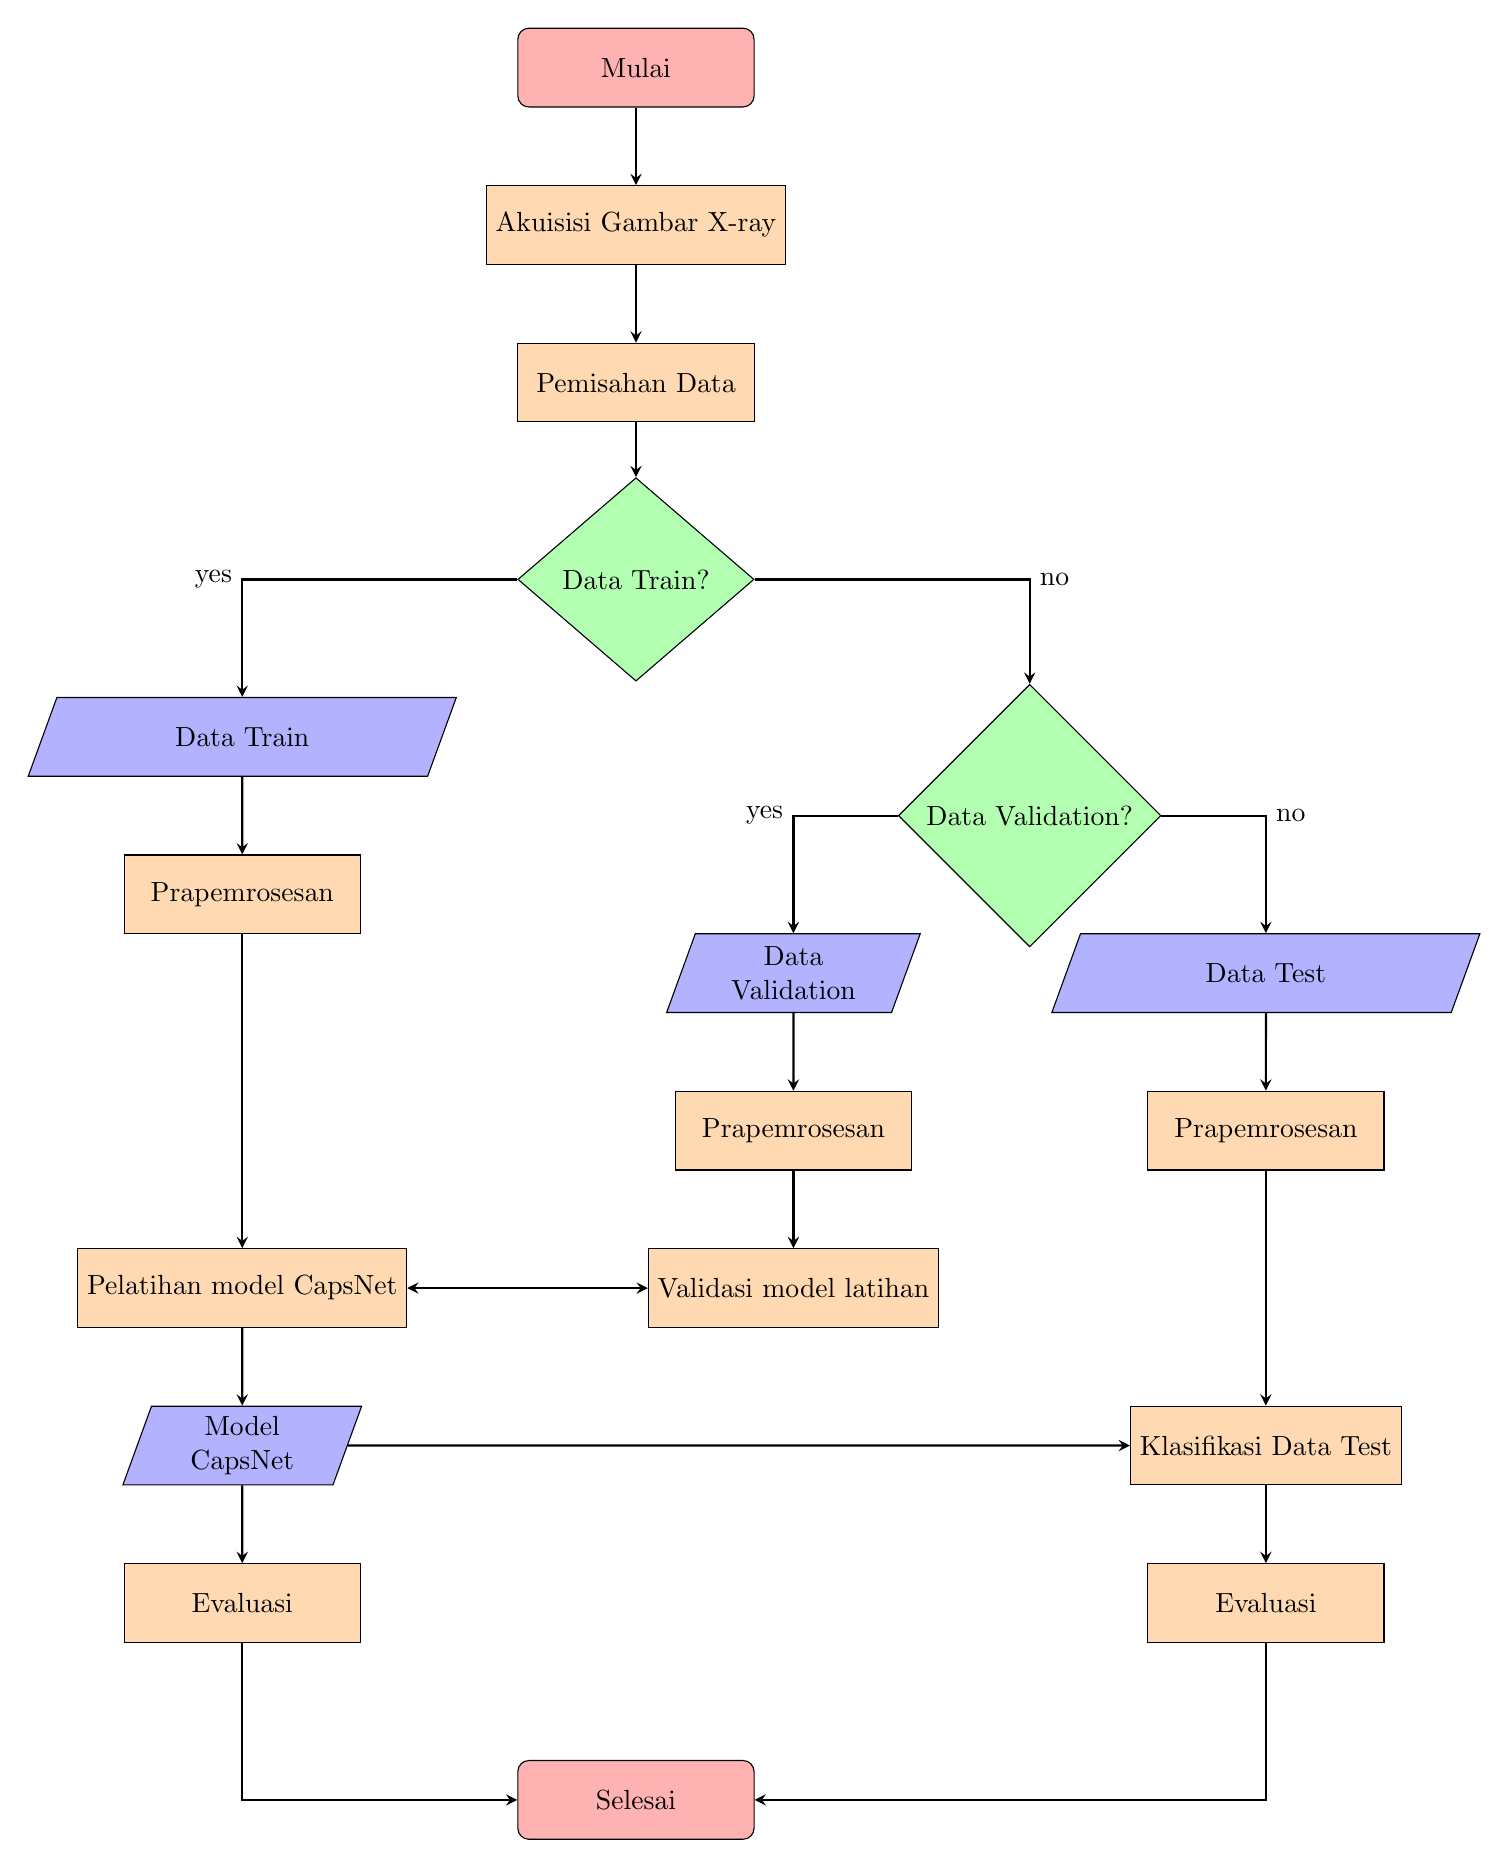
\begin{tikzpicture}[node distance=2cm]
   	
   	\node (start) [startstop] {Mulai};
   	\node (pro1) [process, below of=start] {Akuisisi Gambar X-ray};
   	\node (pro2) [process, below of=pro1] {Pemisahan Data};
   	\node (dec1) [decision, below of=pro2, yshift=-0.5cm] {Data Train?};
   	
   	\node (in1) [io, left of=dec1, xshift=-3cm, yshift=-2cm] {Data Train};
   	\node (pro-a1) [process, below of=in1] {Prapemrosesan};
   	\node (pro-a2) [process, below of=pro-a1, yshift=-3cm] {Pelatihan model CapsNet};
   	\node (out1) [io, below of=pro-a2] {Model CapsNet};
   	\node(pro-a3) [process, below of=out1] {Evaluasi};
   	
   	\node (dec2) [decision, right of=dec1, xshift=3cm, yshift=-3cm] {Data Validation?};
   	
   	\node (in2) [io, left of=dec2, xshift=-1cm, yshift=-2cm] {Data Validation};
   	\node (pro-b1) [process, below of=in2] {Prapemrosesan};
   	\node (pro-b2) [process, below of=pro-b1] {Validasi model latihan};
   	
   	\node (in3) [io, right of=dec2, xshift=1cm, yshift=-2cm] {Data Test};
   	\node (pro-c1) [process, below of=in3] {Prapemrosesan};
   	\node (pro-c2) [process, below of=pro-c1, yshift=-2cm] {Klasifikasi Data Test};
   	\node (pro-c3) [process, below of=pro-c2] {Evaluasi};
   	
   	\node (stop) [startstop, below of=start, yshift=-20cm] {Selesai};
   	
   	\draw [arrow] (start) -- (pro1);
   	\draw [arrow] (pro1) -- (pro2);
   	\draw [arrow] (pro2) -- (dec1);
   	\draw [arrow] (in1) -- (pro-a1);
   	\draw [arrow] (pro-a1) -- (pro-a2);
   	\draw [arrow] (pro-a2) -- (out1);
   	\draw [arrow] (out1) -- (pro-a3);
   	\draw [arrow] (pro-a3) |- (stop);
   	\draw [arrow] (in2) -- (pro-b1);
   	\draw [arrow] (pro-b1) -- (pro-b2);
   	\draw [arrow] (in3) -- (pro-c1);
   	\draw [arrow] (pro-c1) -- (pro-c2);
   	\draw [arrow] (pro-c2) -- (pro-c3);
   	\draw [arrow] (pro-c3) |- (stop);
   	\draw [arrow] (out1) -- (pro-c2);
   	\draw [double-arrow] (pro-a2) -- (pro-b2);
   	\draw [arrow] (dec1) -| node[anchor=east]{yes}(in1);
   	\draw [arrow] (dec1) -| node[anchor=west]{no}(dec2);
   	\draw [arrow] (dec2) -| node[anchor=east]{yes}(in2);
   	\draw [arrow] (dec2) -| node[anchor=west]{no}(in3);
   	
   	\end{tikzpicture}
   	\caption{Diagram alur implementasi penambangan data}
    \end{center}
	\end{figure}
	\begin{figure}[H]
		\centering{\includegraphics[width=\linewidth]{./images/arsitektur/arsitektur_fig1.png}}
		\caption{Arsitektur CapsNet}
		\label{arsitektur_1}
	\end{figure}
	\begin{figure}[H]
		\centering{\includegraphics[width=300px, height=170px]{./images/arsitektur/arsitektur_fig2.png}}
		\caption{Arsitektur Decoder Network}
		\label{arsitektur_2}
	\end{figure}
	\subsection{Arsitektur CapsNet}
	Arsitektur CapsNet yang digunakan dalam makalah ini terdiri dari :
	\begin{enumerate}
		\item \textit{Input Layer}\\
		\textit{Input} menggunakan gambar berukuran 224x224 dengan 3 \textit{channel} yaitu \textit{channel red, green,} dan \textit{blue} atau biasa disebut dengan RGB.
		
		\item \textit{Convolutional Layer 1}\\
		\textit{Layer} ini akan melakukan operasi konvolusi pada gambar \textit{input} menggunakan \textit{out channel} atau \textit{filter} sebanyak 256 dengan \textit{kernel} berukuran 25x25 dan \textit{stride} sebanyak 2. Layer ini akan menghasilkan \textit{feature map}.
		
		\item \textit{Primary Capsule}\\
		\textit{Layer} ini akan mengubah hasil konvolusi menjadi \textit{capsule-capsule}. \textit{Layer} ini terdiri dari beberapa layer, yaitu:
		\begin{itemize}
			\item \textit{Convolution Layer 2}\\ 
			\textit{Layer} ini mendapatkan \textit{input channel} sebanyak 256, lalu operasi konvolusi pada \textit{layer} ini menggunakan \textit{out channel} sebanyak 256 dengan \textit{kernel} berukuran 25x25  dan \textit{stride} sebanyak 16.
			
			\item \textit{Reshape}\\
			Operasi \textit{reshape} digunakan untuk mendapatkan 32x5x5 \textit{capsule} berdimensi 8 setiap \textit{capsule}-nya.
			
			\item \textit{Squash}\\
			\textit{Layer squash} adalah \textit{layer} aktivasi dari primary capsule yang mengubah panjang vektor besar menjadi mendekati 1 dan vektor kecil menjadi 0.
		\end{itemize}
		
		\item \textit{Capsule Layer 1}\\
		\textit{Layer} ini mendapatkan \textit{input capsule} sebanyak 800 berdimensi 8 untuk setiap \textit{capsule}. Lalu algoritma \textit{Routing-by-agreement} akan dijalankan pada layer ini dan menghasilkan \textit{output capsule} sebanyak 32 berdimensi 12 untuk setiap \textit{capsule}.
		
		\item \textit{Capsule Layer 2}\\
		\textit{Layer} ini mendapatkan \textit{input capsule} sebanyak 32 berdimensi 12 untuk setiap \textit{capsule}. Lalu algoritma \textit{Routing-by-agreement} akan dijalankan pada layer ini dan menghasilkan \textit{output capsule} sebanyak jumlah \textit{class} yaitu 3 dan berdimensi 16 untuk setiap \textit{capsule}.
		
		\item \textit{Decoder Network}\\
		\textit{Decoder Network} adalah \textit{layer} yang digunakan CapsNet untuk menghitung \textit{loss} dan melakukan proses rekonstruksi gambar. \textit{Decoder Network} terdiri dari:
		\begin{itemize}
			\item \textit{Fully Connected Layer 1}\\
			\textit{Layer} ini mendapatkan \textit{input} sebanyak jumlah \textit{output capsule} dikali dimensi \textit{capsule} dari \textit{layer} sebelumnya yaitu 3x16 dan menghasilkan 512 \textit{output neuron}. Fungsi aktivasi yang digunakan pada layer ini adalah ReLu.
			
			\item \textit{Fully Connected Layer 2}\\
			\textit{Layer} ini mendapatkan \textit{input} sebanyak jumlah \textit{output neuron} dari \textit{layer} sebelumnya yaitu 512 dan menghasilkan 1024 \textit{output neuron}. Fungsi aktivasi yang digunakan pada layer ini adalah ReLu.
			
			\item \textit{Fully Connected Layer 3}\\
			\textit{Layer} ini mendapatkan \textit{input} sebanyak jumlah \textit{output neuron} dari \textit{layer} sebelumnya yaitu 1024 dan menghasilkan \textit{output neuron} sebanyak ukuran gambar \textit{input} yaitu 224x224x3. Fungsi aktivasi yang digunakan pada layer ini adalah \textit{sigmoid}.
		\end{itemize}
		
	\end{enumerate}
   \newpage
   \section{Analisis}
    \subsection{Analisis \textit{Exploratory Data Analysis}}
     	
	    \begin{figure}[H]
	    	\centering
	    	\includegraphics[width=300px]{/grafik eda/gender.png}
	    	\caption{Grafik perbandingan jenis kelamin}
	    \end{figure}
    	\par Dalam dataset jumlah pasien COVID-19 pria jauh melebihi jumlah pasien wanita.
    	
		\begin{figure}[H]
			\centering
			\includegraphics[width=200px]{/grafik eda/umur.png}
			\includegraphics[width=200px]{/grafik eda/umur2.png}
			\caption{Grafik perbandingan umur}
		\end{figure}
		\par Distribusi umur menunjukkan bahwa sebagian besar pasien berusia paruh baya dengan terpusat pada kisaran umur 50-80. Tidak ada perbedaan signifikan antara distribusi umur pasien pria dan pasien wanita.
		
		\begin{figure}[H]
			\centering
			\includegraphics[width=300px]{/grafik eda/suhu.png}
			\caption{Grafik perbandingan suhu tubuh}
		\end{figure}
		\par Grafik menunjukkan bahwa terdapat perbedaan jarak interkuartil antara pasien yang selamat dan pasien yang meninggal. Pasien yang selamat menunjukkan suhu tubuh sebagian besar di antara 37.75-39.0 derajat celcius, sedangkan pasien yang meninggal menunjukkan jarak yang lebih kecil antara 38.25-38.75 derajat celcius. Pasien-pasien yang masih dirawat sehingga kondisi keselamatannya masih belum diketahui memiliki suhu median yang lebih rendah dibandingkan pasien yang sudah dipastikan status keselamatannya. Hal ini mungkin menunjukkan bahwa pasien-pasien yang baru masuk dan masih dirawat sudah dapat ditangani dengan lebih baik sehingga suhu tubuh pasien secara keseluruhan menurun.
		
		\begin{figure}[H]
			\centering
			\includegraphics[width=200px]{/grafik eda/po2.png}
			\caption{Grafik distribusi angka pO2}
			\includegraphics[width=200px]{/grafik eda/leukosit.png}
			\caption{Grafik distribusi jumlah leukosit}
			\includegraphics[width=200px]{/grafik eda/limfosit.png}
			\caption{Grafik distribusi jumlah limfosit}
			\includegraphics[width=200px]{/grafik eda/neutrofil.png}
			\caption{Grafik distribusi jumlah neutrofil}
		\end{figure}
		\par Saturasi PO2 pasien COVID-19 berada di kisaran 50-100 dengan sebagian besar berada di kisaran 90-100. Angka leukosit pasien berada di kisaran 2.5-11.0 dengan terpusat di angka 7.5. Angka limfosit pasien berada di kisaran 0.2-1.75 dengan sebagain besar berada di sekitar angka 0.75. Angka neutrofil pasien terpisah menjadi dua daerah, dimana sebagian pasien yang memiliki angka neutrofil diantara 1.8-3.0 dan sebagian pasien memiliki angka neutrofil diantara 4.2-5.8.
		
		
		\begin{figure}[H]
			\centering
			\includegraphics[width=300px]{/grafik eda/correlation.png}
			\caption{Grafik Heatmap korelasi fitur}
		\end{figure}
		\par Heatmap korelasi fitur menunjukkan bahwa keselamatan pasien sangat ditentukan oleh umur, dimana umur yang lebih tinggi akan menurunkan kemungkinan keselamatan pasien. Suhu tubuh terlihat tidak memiliki korelasi yang signifikan dengan keselamatan pasien, ditunjukkan dengan warna ungu yang memberi arti korelasi dekat dengan 0. Tingkat saturasi PO2 terlihat memiliki korelasi positif yang cukup signifikan dengan tingkat keselamatan pasien, dimana pasien dengan saturasi PO2 tinggi memiliki kemungkinan lebih tinggi untuk selamat. 
    	
   	\subsection{Analisis Hasil Model CapsNet}
   		\subsubsection{Analisis Metrik Penilaian}   			
   			\begin{figure}[H]
   				\centering
   				\includegraphics[scale=1]{analisis model/final_acc.eps}
   				\caption{Grafik akurasi data validasi}
   			\end{figure}
   			
   			\par Grafik akurasi data validasi menunjukkan fluktuasi besar di 5 \textit{epoch} pertama, karena nilai-nilai awal pada matriks beban model bersifat acak sehingga model belum bisa membuat prediksi dengan akurat. Untuk \textit{epoch} ke 10 dan seterusnya, akurasi validasi model sudah stabil dengan akurasi sekitar 90 \%. Akurasi tes yang hanya sedikit kurang dari akurasi validasi akhir membuktikan bahwa model dapat generalisasi dengan baik pada data yang belum pernah dilihatnya. Hasil akurasi validasi di \textit{epoch} terakhir latihan tercatat pada angka 95.56 \%, sedangkan akurasi pada dataset \textit{test} tercatat pada angka 94.29 \%.
   			
   			\begin{figure}[H]
   				\centering
   				\includegraphics[scale=1]{analisis model/final_acc_norm.eps}
   				\caption{Grafik perbandingkan akurasi data validasi dengan tambahan proses normalisasi}
   			\end{figure}
   			
   			\par Bila proses normalisasi diaplikasikan ke gambar masukan, akurasi validasi model sedikit berkurang. Normalisasi pada gambar masukan berguna pada model CNN sebab model CNN belajar dengan secara terus-menerus menambahkan gradien \textit{error vector} dikalikan dengan \textit{learning rate} ke berbagai matriks beban. Bila vektor masukan tidak dinormalisasi, maka jarak distribusi nilai-nilai fitur akan berbeda untuk setiap fitur, sehingga hasil kurang maksimal. Namun, tampaknya normalisasi tidak membantu meningkatkan performa model CapsNet, melainkan sedikit menurunkan performanya.
   			\par
   			Hal ini terjadi karena 
   			CapsNet memiliki keunggulan dapat menyimpan data positional gambar, maka CapsNet memiliki kemampuan baik ketika gambar terkena transformasi affine atau 
   			transformasi yang dapat mengakibatkan perubahan.\par
   			Ini dapat ditunjukan ketika terjadi transformasi normalisasi CNNs mendapatkan keuntungan sedangkan CapsNet tidak diuntungkan. Jadi kami berkesimpulan
   			bahwa normalisasi pada model dalam makalah ini tidak dapat membantu.
   			
   			\begin{figure}[H]
   				\centering
   				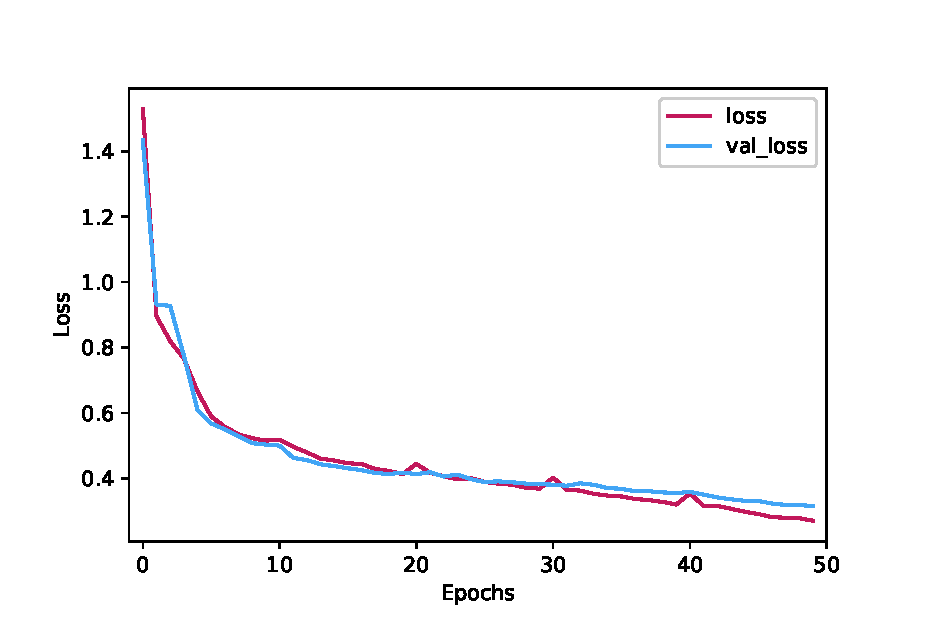
\includegraphics[scale=1]{analisis model/final_loss.eps}
   				\caption{Grafik penurunan fungsi \textit{loss} model}
   			\end{figure}
   			
   			\par Nilai fungsi \textit{loss} dari model terlihat menurun drastis pada 10 \textit{epoch} pertama, lalu menurun secara perlahan di \textit{epoch-epoch} berikutnya. \textit{Loss} pada model ketika latihan dan\textit{loss} pada validasi terlihat mendekati satu sama lain, membuktikan bahwa model tidak mengalami \textit{overfit}.
   			
   			\begin{figure}[H]
   				\centering
   				\includegraphics[scale=1]{analisis model/covid_learn_acc.eps}
   				\caption{Grafik akurasi validasi kasus COVID-19}
   			\end{figure}
   			
   			\par Akurasi validasi untuk khusus kasus-kasus COVID-19 terlihat fluktuatif sampai \textit{epoch} ke 60. Pada \textit{epoch} ke 61 dan seterusnya, kami mencoba memasukan lebih banyak gambar-gambar kasus COVID-19 untuk menambahkan informasi yang didapat oleh model. Hasilnya adalah akurasi validasi model mulai lebih stabil di sekitar 95 \%, dan akurasi tes model untuk kasus-kasus COVID-19 tercatat dengan akurasi sekitar 94 \%.
   			
   			\begin{table}[H]
   			\begin{center}
   				\begin{tabular}{|c|c|c|c|}
   					\hline
   					& \textit{Normal (Predicted)} & \textit{Pneumonia (Predicted)} & \textit{Covid (Predicted)} \\
   					\hline
   					\textit{Normal (Actual)} & 292 & 24 & 1 \\
   					\hline
   					\textit{Pneumonia (Actual)} & 30 & 821 & 3 \\
   					\hline
   					\textit{Covid (Actual)} & 4 & 10 & 77 \\
   					\hline
   				\end{tabular}
   				\caption{Tabel \textit{confusion matrix} model}
   			\end{center}
   			\end{table}
   			
   			\par Hasil \textit{confusion matrix} model akhir menunjukkan bahwa model dapat dengan tepat mengklasifikasikan 77 dari 91 kasus COVID-19. Dari 1171 kasus-kasus yang bukan COVID-19, model hanya mengklasifikasikan secara salah 4 kasus sebagai kasus COVID-19. 
   			
   			\begin{table}[H]
   			\begin{center}
   				\begin{tabular}{|c|c|c|c|}
   					\hline
   					& \textit{Precision} & \textit{Recall} & \textit{F1-score} \\
   					\hline
   					\textit{Normal} & 0.90 & 0.92 & 0.91 \\
   					\hline
   					\textit{Pneumonia} & 0.96 & 0.96 & 0.96 \\
   					\hline
   					\textit{Covid} & 0.95 & 0.85 & 0.90 \\
   					\hline
   					\hline
   					\textit{Macro Avg} & 0.94 & 0.91 & 0.92 \\
   					\hline
   					\textit{Weighted Avg} & 0.94 & 0.94 & 0.94 \\
   					\hline
   					\hline
   					\textit{Accuracy} & \multicolumn{3}{|c|}{0.94} \\
   					\hline
   				\end{tabular}
   				\caption{Tabel metrik-metrik penilaian model}
   			\end{center}
   			\end{table}
   			
   			\par Akurasi keseluruhan model tercatat pada angka 94 \%. \textit{Macro average} menghitung nilai rata-rata \textit{precision}, \textit{recall}, dan \textit{F1-score} dari tiap kelas. \textit{Weighted average} menambahkan nilai \textit{precision}, \textit{recall}, dan \textit{F1-score} masing-masing kelas dengan dikalikan beban yang tergantung dengan jumlah kasus benar dari tiap kelas. Terlihat bahwa \textit{weighted average} dari \textit{precision}, \textit{recall}, dan \textit{F1-score} bernilai konsisten dengan akurasi keseluruhan, yaitu 94 \%.
   		
   		\subsubsection{Hasil Rekonstruksi}
		\par
		Hasil prediksi pada \textit{Dense Capsule 2} diteruskan kepada \textit{Decoder Network} menghasilkan rekonstruksi gambar dimana hasil ini akan dipakai sebagai $L_{2}$/ \textit{Reconstruction Loss}. Metode hasil rekonstruksi sebagai \textit{loss function} ini digunakan untuk menggeneralisasi data mencegah \textit{overfitting} dengan mendorong \textit{Capsules} untuk dapat \textit{encode} fitur-fitur yang terdapat pada input gambar.
		\begin{figure}[H]
			\centering
			\includegraphics[width=0.7\textwidth]{./images/"contoh dataset"/Normal}
			\caption{Gambar Chest X-Ray Normal (atas) dengan Rekonstruksi (bawah).}
		\end{figure}
		\begin{figure}[H]
			\centering
			\includegraphics[width=0.7\textwidth]{./images/"contoh dataset"/Pneu}
			\caption{Gambar Chest X-Ray Pneumonia (atas) dengan Rekonstruksi (bawah).}
		\end{figure}
		\begin{figure}[H]
			\centering
			\includegraphics[width=0.7\textwidth]{./images/"contoh dataset"/Cov}
			\caption{Gambar Chest X-Ray COVID-19 (atas) dengan Rekonstruksi (bawah).}
		\end{figure}
		\par
		Dari hasil rekonstruksi gambar pada figur diatas, walaupun input gambar memiliki perbedaan seperti lebih besar, memiliki kemiringan atau transformasi affine lain. Hasil rekonstruksi akhir model dapat tetap menjaga struktur fitur input gambar awal. Hasil rekonstruksi secara samar memiliki bentuk, struktur dan fitur-fitur yang menyerupai input gambar awal.
   \newpage
   \section{Kesimpulan}
    Di era digital sekarang ini, kemampuan algoritma \textit{Deep Learning} dapat menyaingi tingkat performa manusia. Tugas manusia memproses data dari suatu gambar sulit dikerjakan oleh komputer, tetapi sekarang dengan kemajuan algoritma dapat dilakukan dengan mesin. Berdasarkan percobaan yang telah kami lakukan, model kami dapat mengklasifikasi perbedaan antara gambar Chest X-Ray normal, pneumonia dan COVID-19 dengan akurasi validasi 0.9556 dan akurasi tes 0.9429.
    \par
    Metode yang kami gunakan untuk masalah di makalah ini mencakup pengumpulan data, prapemrosesan, model CapsNet, dan evaluasi. Langkah-langkah prapemrosesan terdiri dari konversi model warna gambar ke RGB, pemotongan ukuran gambar menjadi 224x224, normalisasi, dan konversi ke PyTorch Tensor. Model CapsNet yang kami gunakan  terdiri dari beberapa lapisan : \textit{input layer}, \textit{convolutional layer 1}, \textit{primary capsule}, \textit{capsule layer 1}, \textit{capsule layer 2}, dan \textit{decoder network}.
    \par
    Studi ini memiliki beberapa kelebihan dan kekurangan. Metode CapsNet tergolong baru sehingga aplikasinya menggunakan teknik-teknik mutakhir. Keadaan dunia masa kini yang sedang berada dalam situasi pandemik COVID-19 juga sangat menyambut inovasi-inovasi teknologi yang dapat membantu tenaga medis. Hasil dari studi juga cukup memuaskan, dimana performa model pada data tes menghasilkan akurasi 0.9429. Salah satu kekurangan dari studi adalah kurangnya jumlah data gambar X-Ray dada pasien COVID-19 yang tersedia secara umum, sehingga performa model kurang maksimal. Gambar X-Ray dada pasien COVID-19 yang tersedia juga semuanya berasal dari luar Indonesia, sehingga performa model belum dapat dites pada gambar X-Ray dada pasien dari Indonesia. 
    \par
    Pihak yang dapat mendapatkan manfaat dari penelitian ini adalah tenaga medis yang sedang menangani kasus-kasus COVID-19. Aplikasi dari model dari makalah ini dapat menyediakan opini kedua yang meningkatkan kepastian dari hasil metode-metode deteksi COVID-19 lain seperti \textit{rapid test} dan \textit{swab test}. Model juga dapat digunakan pada fasilitas-fasilitas medis yang memiliki kemampuan mengambil gambar X-Ray dan kekurangan alat-alat tes lain untuk mendeteksi COVID-19. Hasil yang diharapkan adalah model dapat meningkatkan deteksi pasien-pasien yang terjangkit virus COVID-19 secara cepat dan akurat sehingga menghambat penyebaran virus COVID-19 di Indonesia.  
   
   \section{Dokumentasi}
   Hasil dan program dapat ditemukan pada pranala berikut :\url{https://github.com/Yakuy/Gemastik13}
   \newpage
   \printbibliography[title=Daftar Pustaka]

\end{document}